\documentclass[10pt,a4paper]{article}
\usepackage{graphicx}

\begin{document}
\title{Lab 1: Interfacing with the WiiMote}
\author{Sam Mansfield and Toan Voung \\
  EECS149}
\date{September 11th, 2013}
\maketitle

\section*{Introdcution}
  Something goes here.
\section*{Analysis}
  \subsection*{2 Pair a desktop computer with the WiiMote}
    \subsubsection*{a What is the MAC address of your WiiMote?}
      Something goes here.
  \subsection*{3 Plot the uncalibrated accelerometer signal from the WiiMote} 
    \subsubsection*{a What are the values of the x and y axes when the WiiMote is at rest on level ground?}
      Something goes here.
    \subsubsection*{b What is the value of the z axis when the WiiMote is at rest on level ground? What quantity is begin measured?}
      Something goes here.
  \subsection*{4 Control the WiiMote actuators}
    \subsubsection*{a What is the Report ID and Payload to turn WiiMote LEDs 2 and 4 on, and LEDs 1 and 3 off?}
      Something goes here.
    \subsubsection*{b How can you modify the above sequence to also enable the rumble motor?}
      Something goes here.
  \subsection*{5 Measure sensitivity and bias of the accelerometer}
    \subsubsection*{a Where are these measurements stored?}
      Something goes here.
    \subsubsection*{b What bias did you record?}
      Something goes here.
    \subsubsection*{c What sensitivity did you record?}
      Something goes here.
    \subsubsection*{d Provide screenshots of changes to the block diagram code}
      Something goes here.
  \subsection*{6 Calibrate the accelerometer}
    \subsubsection*{a What equations did you use to calibrate the accelerometer and to calculate the magnitude of the acceleration it measures?}
      To calibrate the accelerometer we used a simple affine function and the assumptions that when the WiiMote is at rest, with the buttons facing upwards, the callibrated x and y will be 0 and the callibrated z will be 1: 
        \[callibratedX = \frac{x - bias}{sensitivity}\] 
        \[callibratedY = \frac{y - bias}{sensitivity}\] 
        \[callibratedZ = \frac{z - bias}{sensitivity}\] 
      And at rest:
        \[callibratedX = \frac{x - bias}{sensitivity} = 0\] 
        \[callibratedY = \frac{y - bias}{sensitivity} = 0\] 
        \[callibratedZ = \frac{z - bias}{sensitivity} = 1\] 
      So solving for bias we get:
        \[bias = x\]
        \[bias = y\]
      And since x and y aren't the same value at rest we averaged x and y for the bias:
        \[bias = \frac{x + y}{2}\]
      To calculate sensitivity we used the following formula:
        \[sensitivity = z - bias\]
      Substituting in bias we get:
        \[sensitivity = z - \frac{x + y}{2}\]
      To solve for magnitude we used the distance formula:
        \[magnitude = \sqrt{x^2 + y^2 + z^2}\]
    \subsubsection*{b Based on your calibration parameters and the number of bits of resolution of the WiiMote ADC, and an affine model of the WiiMote accelerometer, what is your estimate of the maximum acceleration that the WiiMote can measure?}
      The maximum acceleration is when x, y, and z are at their max. It appeared that the max uncalllibrated value of x, y, and z was 256, which would be 8 bits. This gives a max callibrated x, y, and z of:
        \[callibratedXMAX = \frac{256 - bias}{sensitivity} = 0\] 
        \[callibratedYMAX = \frac{256 - bias}{sensitivity} = 0\] 
        \[callibratedZMAX = \frac{256 - bias}{sensitivity} = 1\]
      Substituting in bias and sensitivity:
        \[callibratedXMAX = \frac{256 - 124}{26} \approx 5\] 
        \[callibratedYMAX = \frac{256 - 124}{26} \approx 5\] 
        \[callibratedZMAX = \frac{256 - 124}{26} \approx 5\]
    \subsubsection*{c When the WiiMote is at rest, what should be the value of the magnitude indicator?}
      At rest the only acceleration is gravity. Since we are measuring magnitude in g-forces, it should be 1g. 
    \subsubsection*{d Why is it better to perform calibration at runtime, rather than hard-coding values for the sensitivity and bias of the sensor?}
      The problem with hardcoding values for bias and sensitivity is that you are assuming that the WiiMote will always produce the same uncallibrated values for x, y, and z, which is not a stable assumption. The uncallibrated values can be dependent on temperature, which WiiMote you are using, and age of the WiiMote. 
    \subsubsection*{e Provide the relevant MathScript code and screenshots of changes (if any) to the block diagram}
    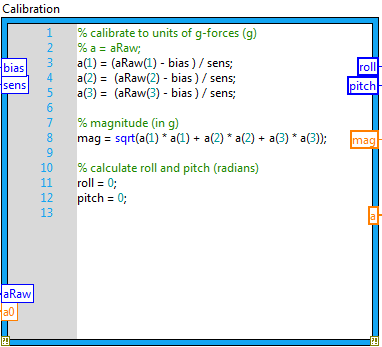
\includegraphics{../lab1_data/lab1_6e.PNG} 
  \subsection*{7 Measure Pitch and Roll}
    \subsubsection*{a What equations did you use to calculate pitch and roll?}
      We used these two equations to calculate pitch and roll:
        \[pitch = \arctan(\frac{y}{\sqrt{x^2 + z^3}})\]
        \[roll = \arctan(\frac{-x}{z})\]
    \subsubsection*{b Provide the relevant MathScript code and screenshots of changes (if any) to the block diagram.}
    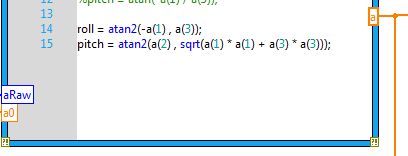
\includegraphics{../lab1_data/lab1_7a.PNG} \\[1em] 
    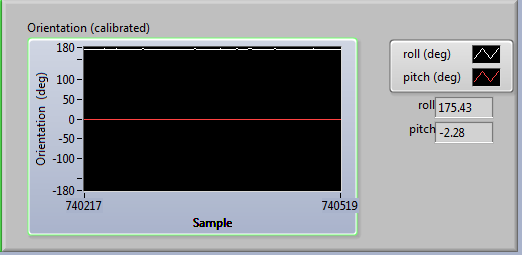
\includegraphics{../lab1_data/lab1_7b.PNG} 
  \subsection*{8 Filter the accelerometer signal}
    \subsubsection*{a Describe your filter, and include an equation for its impulse response, frequency response, or its output as a fraction of input.}
      We used a averaging low pass filter of the form:
        \[Filter(x) = (1 - q)*callibratedX(x) + q*callibratedX(x-1)\]
        \[Filter(y) = (1 - q)*callibratedY(y) + q*callibratedY(y-1)\]
        \[Filter(z) = (1 - q)*callibratedZ(z) + q*callibratedZ(z-1)\]
      We varied the q from 0.5 to 0.99 and decided that 0.9 provided the best response. The signal was less noisy and the delay was still low. This was a good compromise. 
      The impulse response of our filter was:
        \[h(n) = q^n*U(n)\]
      And our frequency response was:
        \[H(z) = \frac{q}{1 - (1 - q)*z^{-1}}\]
    \subsubsection*{b Provide the relevant MathScript codd and screenshots of changes (if any) to the block diagram}
      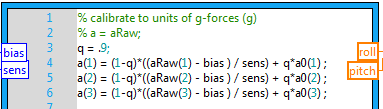
\includegraphics{../lab1_data/lab1_8a.PNG} 
  \subsection*{9 Share Your Feedback}
    This was an overall straightforward and helpful lab.
\section*{Conclusion}
  This lab helped us to go through the process of receiving unfiltered data from a standard embedded system (WiiMote), and using that data to produce meaningful data, such as a callibrated accelerometer with magnitude. It was helpful to go through the process of figuring out how to calculate the bias and sensitivity without hardcoding the values, which is an extremely good way to think about calibration. It would have been nice to do a little more interfacing with the WiiMote, such as with the turning on and off different features and looking how the data is coming in byte wise and filtering it based on its significance.
  
  Overall the lab covered a broad range of ideas from basic algebra (calculating bias and sensitivity), vector analysis (calculating magnitude, pitch, and roll), and signal analysis (filtering the accelerometer signal). All these skills were simple, but also complicated since we had to pull from different sections of our brain, which was a great exercise. 
\end{document}

